\graphicspath{{figures/static/}}
\chapter{输电塔在龙卷风作用下的静态响应分析}
\section{龙卷风风场处理}
输电塔在龙卷风风场中的水平投影示意图如图\ref{fig:tower-tornado-cs}所示。
\begin{figure}[!htpb]
  \centering
  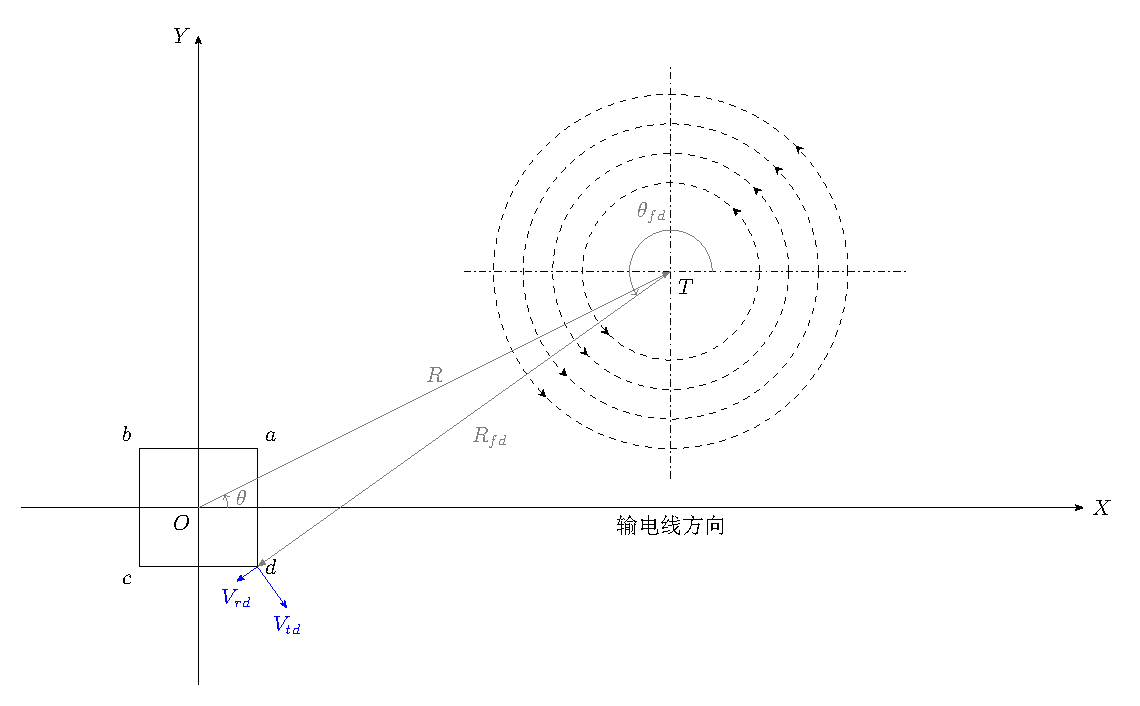
\includegraphics[width=\textwidth]{tower_tornado_cs.pdf}
  \caption{输电塔在龙卷风风场中的水平投影示意图}
  \label{fig:tower-tornado-cs}
\end{figure}
输电塔直角坐标系$\{O: XYZ\}$的建立方法见第\ref{sec:tower-fea}节。
$abcd$为输电塔处于同一水平剖面的节点。
下文主要展示推导$d$节点处龙卷风风速的方法,其余节点类似。
龙卷风中心在坐标系$\{O: XYZ\}$中的位置用极坐标$(R, \theta)$表示。
输电塔节点$d$相应于龙卷风核心的极坐标为$(R_{fd}, \theta_{fd})$,$d$节点受到的龙卷风切向、径向风速分别为$V_{td}$、$V_{rd}$,以及图\ref{fig:tower-tornado-cs}未明确表示的竖向风速$V_{ad}$。

\subsection{输电塔节点相应于龙卷风中心位置的极坐标}\label{sec:d-polor}
假设$d$节点在输电塔坐标系$\{O: XYZ\}$中的坐标为$(x_d, y_d, z_d)$,下文将推导节点$d$相应于龙卷风中心的极坐标$(R_{fd}, \theta_{fd})$。

龙卷风中心$T(R, \theta)$在输电塔坐标系$\{O: XYZ\}$中的直角坐标为$(R\cos\theta, R\sin\theta)$,则节点$d$相应于龙卷风中心$T$的向量为:
\begin{equation}
  \vv{Td} = \vv{Od} - \vv{OT} = (x_d - R\cos\theta, y_d - R\sin\theta) = R_{fd}(\cos\theta_{fd}, \sin\theta_{fd})
\end{equation}
式中,
\begin{equation}
\begin{split}
  R_{fd} & = \sqrt{(x_d-R\cos\theta)^2+(y_d-R\sin\theta)^2} \\
  \theta_{fd} & = \arctan \frac{y_d - R\sin\theta}{x_d - R\cos\theta}
\end{split}
\end{equation}

\subsection{龙卷风风场在直角坐标系下的分量}\label{sec:cs}
第\ref{sec:tornado}节模拟的龙卷风风场是定义在极坐标系下的,而施加风荷载采用直角坐标系下的风速分量较为简单,因此需要将龙卷风风场从极坐标系转化为直角坐标系。

输电塔节点$d$受到的龙卷风径向风速$V_{rd}$与$X$轴正方向的夹角为$\theta_{fd}$(图\ref{fig:tower-tornado-cs}),切向风速$V_{td}$与$X$轴正方向的夹角为$(\theta_{fd}+\pi/2)$,进行速度的分解如下:
\begin{equation}
\begin{split}
  V_{xd} & = V_{rd} \cos\theta_{fd} + V_{td} \cos(\theta_{fd}+\pi/2) \\
         & = V_{rd} \cos\theta_{fd} - V_{td} \sin(\theta_{fd}) \\
  V_{yd} & = V_{rd} \sin\theta_{fd} + V_{td} \sin(\theta_{fd}+\pi/2) \\
         & = V_{rd} \sin\theta_{fd} + V_{td} \cos(\theta_{fd}) \\   
  V_{zd} & = V_{ad}  
\end{split}
\end{equation}

有了上述准备工作,就可以计算输电塔上任意节点受到的龙卷风风速在直角坐标系下的分量了。

\subsection{龙卷风风场中任意节点处风速分量}
输电塔节点$d$相应于龙卷风中心的实际位置为$(R_{fd}, \theta_{fd})$(见第\ref{sec:d-polor}节),此节点对应于缩尺龙卷风风场$V_r(r,z)$、$V_t(r,z)$和$V_a(r,z)$(见第\ref{sec:tornado}节)中的位置为$(R_{md}, Z_{md})$,且
\begin{equation}
\begin{split}
  R_{md} & = R_{fd} / L_s \\
  Z_{md} & = z_{fd} / L_s
\end{split}
\end{equation}

在缩尺龙卷风风场中,由位置$(R_{md}, Z_{md})$可提取缩尺龙卷风风场径向、切向和竖向风速分量分别为$V_{rmd}$、$V_{tmd}$和$V_{amd}$。根据缩尺龙卷风速度相似比$V_s$可将其转化为足尺龙卷风风场中的速度分量:

\begin{equation}
\begin{split}
  V_{rd} &= V_{rmd} \times V_s \\
  V_{td} &= V_{tmd} \times V_s \\
  V_{ad} &= V_{amd} \times V_s
\end{split}
\end{equation}

最后根据第\ref{sec:cs}节的方法即可将输电塔节点$d$受到的极坐标系下的足尺龙卷风风速分量转化为直角坐标系下的风速分量。


\section{龙卷风风荷载计算}


\section{索的悬链线理论及输电线作用于塔的荷载}

\subsection{索的悬链线理论基本假设}
索由高强钢丝集束而成,相对抗弯刚度很小,其受力特点可以认为是完全柔性。
在自重和张力作用下分析其线形和力学参数时,基本假设如下:

\begin{itemize}
  \item
  索是理想柔性,既不能受压也不能受弯;
  \item
  索的材料符合胡克定律;
  \item
  索的横截面积在外荷载作用下的变化量十分微小,可忽略不计。
\end{itemize}

为了确定重力作用下索的线形,以弦左端点为原点、竖直向上为Y轴正方向建立右手直角坐标系。
则索受到的重力沿Y轴负向。
假设单位长度索的质量恒定,且不随张力变化。

\begin{figure}[!htbp]
  \centering
  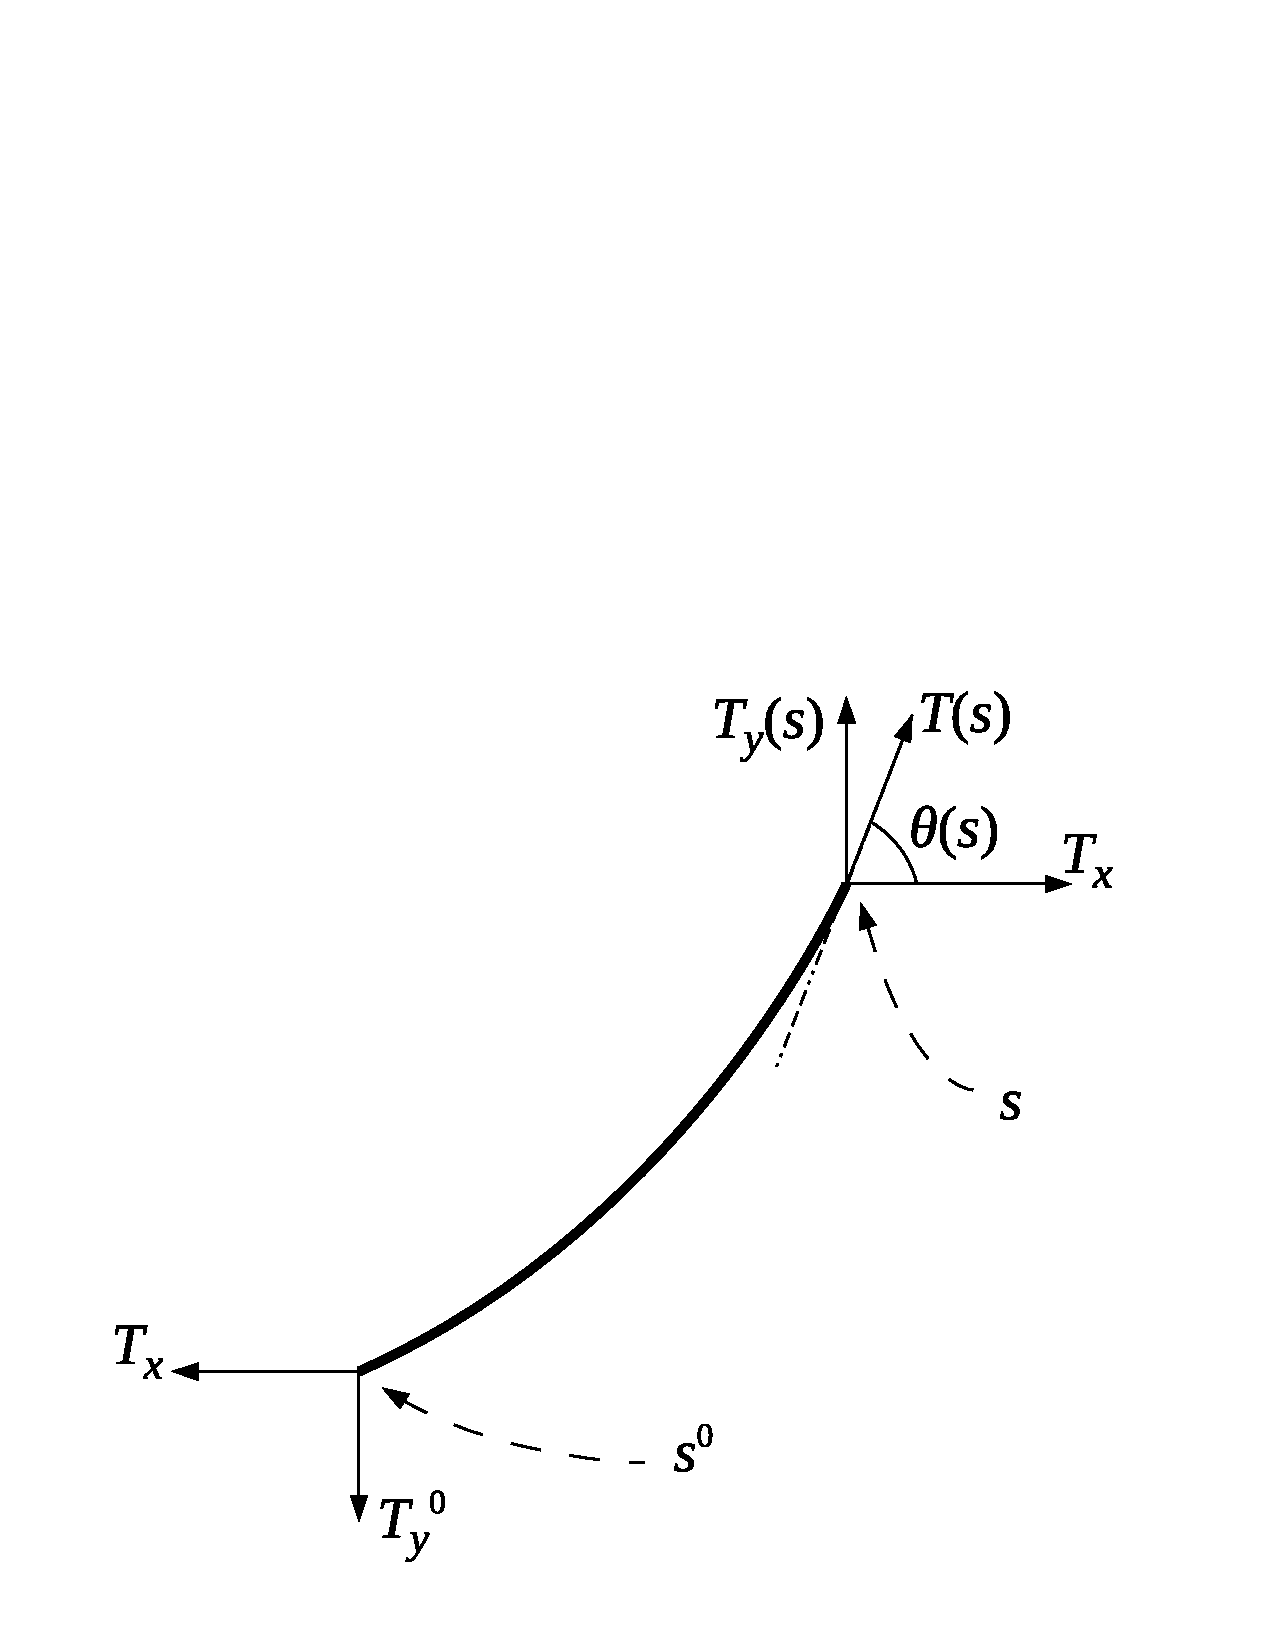
\includegraphics[width=0.6\textwidth]{catenary_diagram.pdf}
  \label{fig:catenary}
  \caption{索段计算示意图}
\end{figure}

\subsection{符号约定}
\begin{description}
  \item[$s$]
  从索左端点(坐标系原点)开始计算的索长度;
  \item[$\mu$]
  单位长度索的质量(假设是恒定的);
  \item[$T(s)$]
  索长度为$s$处的索张力(根据柔性索假设,张力沿索的切线方向);
  \item[$T_y(s)$]
  索长度为$s$处的索张力的$Y$向分量;
  \item[$T_x$]
  张力的$X$向分量(任取索段进行受力分析,由$X$向平衡方程可知$T_x$沿索长是均匀的);
  \item[$\theta(s)$]
  索切向量与$X$轴正向的夹角。
\end{description}

\subsection{自重作用下的单索线形求解}
索段竖向的平衡方程为:
\begin{gather}
  T_y(s) = g \int_{s^0}^{s} \mu \mathrm{d}s + T_y^0 \notag \\
  T_x \tan(\theta(s)) = g \mu \int_{s^0}^{s} \mathrm{d}s + T_y^0 \notag \\
  T_x \frac{\mathrm{d} y}{\mathrm{d} x} = g \mu \int_{s^0}^{s} \sqrt{1+\left(\frac{\mathrm{d} y}{\mathrm{d} x}\right)^2} \mathrm{d}x + T_y^0 \notag \\
  \frac{\mathrm{d}^2 y}{\mathrm{d} x^2} = \frac{g \mu}{T_x} \sqrt{1+\left(\frac{\mathrm{d} y}{\mathrm{d} x}\right)^2}
\end{gather}
此二阶微分方程的解析解为:
\begin{equation}
  y = \frac{T_x}{g \mu} \cosh \left( \frac{g \mu}{T_x} + c_1 \right)+c_2
\end{equation}
式中,$c_1$和$c_2$为由边界条件确定的积分常量。代入边界条件:$x=0,y=0;x=L,y=C$(见图\ref{fig:cat})。

\begin{figure}[!htpb]
\centering
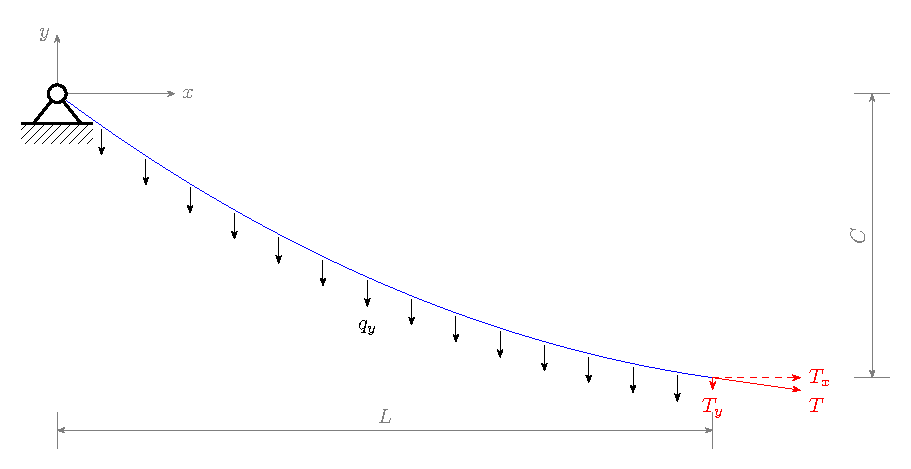
\includegraphics[width=0.8\textwidth]{cat.pdf}
\caption{单缆尺寸及边界条件示意图}
\label{fig:cat}
\end{figure}

\begin{equation}
  \left \{
    \begin{split}
      & \beta = \frac{g \mu L}{2 T_x}\\
      & c_1 = \sinh^{-1}\left(\frac{\beta C / L}{\sinh \beta}\right)\\
      & c_2 = -\frac{T_x}{g \mu} \cosh(c_1)
    \end{split}
  \right.
\end{equation}

悬链线索的形状长度$S$和无应力长度$S_0$分别为:
\begin{equation}
  S = \frac{T_x}{g\mu}\left[\sinh\left(\frac{g \mu L}{T_x}+c_1\right)+\sinh(c_1)\right]
\end{equation}

\begin{equation}
\begin{split}
  S_0 &= S-\Delta S \\
      &= S - \frac{T_x}{EA g \mu }\left[ \frac{1}{2} g \mu L + \frac{1}{8} T_x \left( e^{2(c_1+2\beta)} - e^{-2(c_1-2\beta)} -e^{2c_1} + e^{-2c_1} \right) \right]
\end{split}
\end{equation}

\subsection{输电线施加在输电塔的荷载求解}

跨越塔之间输电线跨度为$L=\SI{1770}{m}$,右侧支座比左侧支座高度相同,即$C=\SI{0}{}$,跨中矢高$f=\SI{132.4}{m}$,单位长度质量$\mu=\SI{3219}{kg/km}$。
索的弹性模量$E=\SI{108070}{MPa}$,截面积$A=\SI{729}{mm^2}$。
假设在外荷载作用下两支座的间距及高差保持不变。
主要任务是利用上述悬链线理论计算输电线对输电塔施加的荷载。

主要思路:输电线在自重和张力作用下,其线形为悬链线,故可采用悬链线经典公式来进行求解。
采用直接建模的方式,单缆采用LINK1单元模拟,单元水平长度为\SI{1}{m}。
分析时,首先假定水平力大小,根据悬链线方程求解节点坐标,由此建立节点和单元,并分析单缆在自重作用下的内力和线形。
如果求解获得的水平力与假定水平力之间的误差较大或者单缆变形较大,则返回重新计算,直至满足误差要求。计算框图如图\ref{fig:flow-chart}所示。
\begin{figure}[!htpb]
\centering
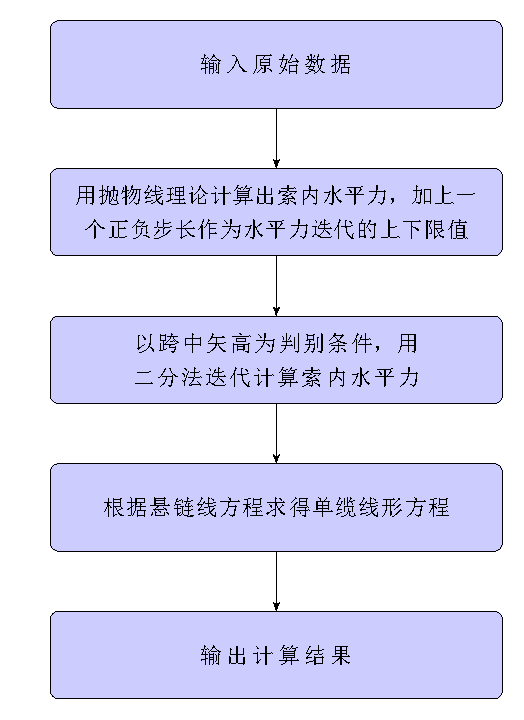
\includegraphics[width=0.4\textwidth]{flow_chart.pdf}
\caption{单缆线形和力学参数计算框图}
\label{fig:flow-chart}
\end{figure}

计算的APDL和MATLAB程序见附录\ref{apen:cat}。如图\ref{fig:cat-disp}所示,\SI{12.7}{mm},相比于跨径$L=\SI{1770}{m}$该变形已足够小,认为已满足精度要求。

\begin{figure}[!htbp]
\centering
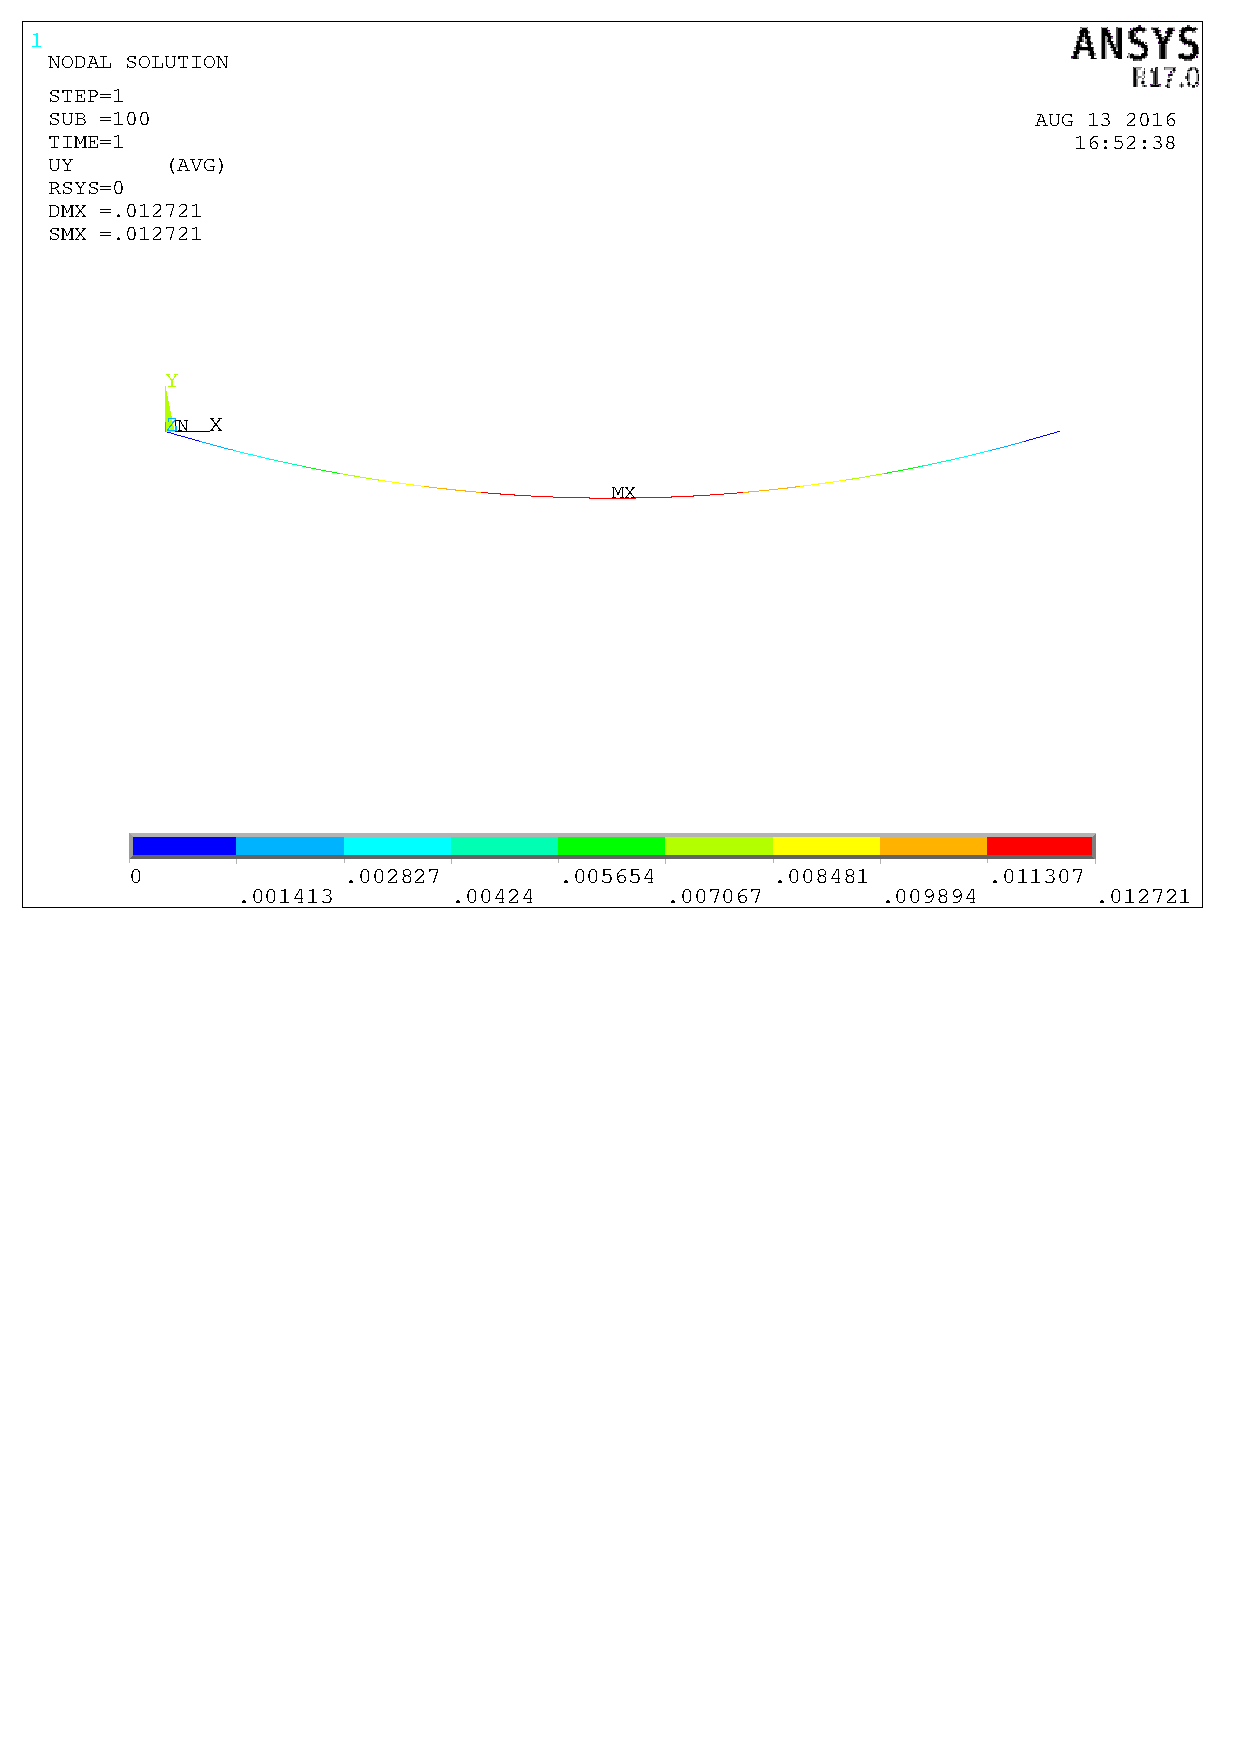
\includegraphics[width=0.6\textwidth]{cat_disp.pdf}
\caption{跨越塔之间输电线变形图(单位:\SI{}{m})}
\label{fig:cat-disp}
\end{figure}

对于跨越塔和锚塔之间的输电线对跨越塔的荷载计算采用相同的方法,在此不一一列举。

跨越塔受到的两侧输电线传来的张力的示意图见图\ref{fig:line-force}所示。

\begin{figure}[!htbp]
\centering
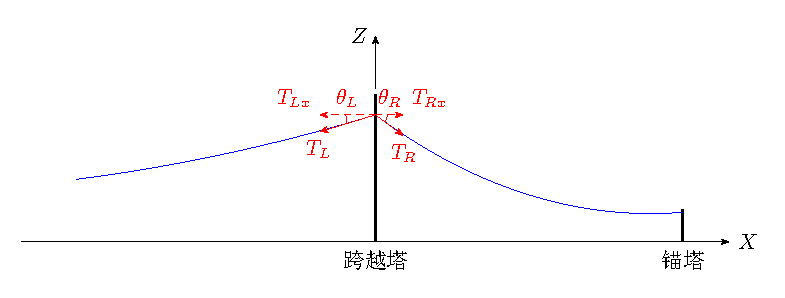
\includegraphics[width=0.8\textwidth]{line_force}
\caption{跨越塔受到输电线的张力示意图}
\label{fig:line-force}
\end{figure}

经过附录\ref{apen:cat}程序的计算,图\ref{fig:line-force}中各量为:
\begin{equation}
\begin{split}
  T_{Lx} & = \SI{93.31}{kN},\quad \theta_L  = \ang{16.89} \\
  T_{Rx} & = \SI{21.33}{kN},\quad \theta_L  = \ang{36.70}
\end{split}
\end{equation}





\section{龙卷风位置变化的参数分析}
